\chapter{QuACKs}
\label{sec:quack}

In a Sidekick connection, a proxy needs to be able to refer to and efficiently
acknowledge a set of packets even when they are randomly encrypted. Since
packets in a TCP connection are labeled with cleartext sequence numbers, it is
straightforward to refer to a set of TCP packets using cumulative and selective
ACKs. But this problem is technically challenging for packets of secure
transport protocols without access to cleartext sequence numbers or the
ossification of other fields.

We mathematically define the quACK problem in the context of network packets
sent over a lossy path segment, and discuss how to select \emph{identifiers} to
refer to encrypted packets. We analyze strawman solutions to the quACK problem
that use either too much space or computation. Then, we present two efficient
constructions of the quACK inspired by related theoretical work in set
reconciliation~\cite{minsky2003set,eppstein2011straggler}, as well as coding
theory and graph theory~\cite{karpovsky2003data}. Both constructions require a
bound on the maximum number of missing elements, a threshold $t$, and have
different tradeoffs. The \textit{power sum} construction is space-optimal and
deterministic, but requires an exact bound. The \textit{invertible Bloom lookup
table (IBLT)} construction is more computationally scalable with an approximate
bound, but also probabilistic with constant factor overheads.

Concretely realized, the power sum quACK uses 48~bytes to express the equivalent
of TCP's cumulative + selective ACK over the 32-bit identifiers of randomly
encrypted packets, tolerating up to 10 missing packets before the last
``selective ACK.'' On a recent x86-64 CPU, it takes 26~ns to encode a single
packet in the power sum quACK, and 15.5~$\mu$s to decode which received packets
the quACK represents. The IBLT quACK takes 42~ns to encode a single packet and
1.3~$\mu$s to decode a quACK, using at least 58~bytes. These overheads compared
well with several alternatives
(\Cref{tab:quack:overview:practical}).

\section{The QuACK Problem}
\label{sec:quack:problem}

In the quACK problem, a sender (such as an endpoint) transmits a
multiset\footnote{A ``multiset'' means the same element can be transmitted more
than once.} of elements $S$. At any given time, a receiver (such as a proxy)
has received a subset $R \subseteq S$ of the sent elements. We would like the
receiver to communicate a small amount of information to the sender, who then
efficiently decodes the missing elements---the set difference $S \setminus
R$---knowing $S$. This small amount of information is called the ``quACK''. The
problem is: \textbf{what is in a quACK and how do we decode it?}

\subsection{Identifiers}
\label{sec:quack:problem:identifiers}

How exactly do we refer to the elements in the quACK problem that have been sent
or received? In a networking context, these elements are packets. Traditional
TCP proxies have been able to interpose their own concise, cumulative
acknowledgments using cleartext sequence numbers, but this is not possible with
modern, secure transport protocols. Even if a connection did expose an
unencrypted numerical field, we would not want to refer to that field at risk
of ossifying that protocol.

Instead, we need a function that deterministically maps
a packet to a random $b$-byte \emph{identifier}. The most trivial solution
that applies to all base protocols is
to hash the entire payload. Another option if the payload is already
pseudorandom (e.g., QUIC) is to take the first $b$ bytes from a fixed
offset of that payload. Although the latter option would rely on those bytes
to remain pseudorandom, it is computationally more efficient because it
does not require reading the entire payload.

\subsubsection{Collisions.}
The main considerations when selecting the number of bytes, $b$, in an
identifier is the tolerance for collisions compared with the extra data
needed to refer to these packets on the link. The larger $b$ is, the lower
the collision probability but the greater the link overhead.

Define the collision probability to be the probability that a randomly-chosen
$b$-byte identifier in a list of $n$ packets maps to more than one packet in
that list.
If we assume that identifiers are uniformly distributed,
this probability is equal to $1-(1 - 1/256^{b})^{n-1}$.
When $n=500$, using $4$ bytes results in an almost negligible
chance of collision while using $2$ bytes results in a 0.8\% chance
(\Cref{tab:quack:collision-prob}).

\begin{table}[ht]
  \centering
  \begin{tabular}{|l|l|l|l|l|}
    \hline
    \textbf{Identifier Bytes} & 1 & 2 & 4 & 8 \\
    \hline
    \textbf{Collision Prob.}
    & 0.090 & 0.0004 & $5.6\text{e-09}$ & ${\approx}0$ \\
    \hline
  \end{tabular}
  \caption{Collision probabilities for $n=25$.
  }
  \label{tab:collision-prob}
\end{table}


When handling collisions, a sender who is decoding a quACK has a list of $n$
packets it is trying to classify as received or missing
(\Cref{sec:quack:constructions}). This is the number of packets that were either
not classified or newly transmitted since decoding a previous quACK.
Note that collisions are also known to the
sender beforehand. If there is a collision between a packet that is received
and a packet that is missing, the fate of that identifier is considered
indeterminate. Either the protocol can still function with approximate
statistics (e.g., congestion control) or it can fall back to an end-to-end
mechanism (e.g., retransmission).

\subsection{Strawman solutions}
\label{sec:quack:problem:strawmen}

A problem that is simple with cumulative and selective acknowledgments of
plaintext sequence numbers is deceivingly challenging for pseudorandom
packet identifiers. Consider the following strawman solutions to the quACK
problem:

\subsubsection{Strawman 1: Echo every identifier.}
Strawman 1a, similar to \cite{li-tsvwg-loops-problem-opportunities-06,kramer2020lwpep},
echoes the identifier of every received packet in a new UDP packet to the data
sender.  Decoding is trivial given that the identifiers are unmodified.
This strawman adds significant link overhead in terms of additional packets.
Additionally, since the strawman is not cumulative, losing a quACK means the
end host could falsely consider a packet to be lost, creating a congestion
event or spurious retransmission.

Strawman 1b echoes a sliding window of identifiers over UDP such that there is
overlap in the identifiers referred to by consecutive quACKs.
This solution is slightly more resilient to loss, but uses more bytes and is
still not guaranteed to be reliable.
Another variant batches identifiers to reduce the number of packets, but this
solution is even less resilient to loss.

We also consider a Strawman 1c that echoes every identifier over TCP with
\texttt{TCP\_NODELAY} to send every identifier in its own packet.
This ensures there are no false positives when detecting lost packets,
but adds even more link overhead in terms of TCP headers and additional ACKs
from the data sender (every other packet by default in the Linux kernel).

\subsubsection{Strawman 2: Cumulative hash of all identifiers.}
Strawman 2 sends a SHA-256 hash of a sorted concatenation of all the received
packets in a UDP packet, and the sender hashes every subset of the same size of
sent packets until it finds the subset with the same hash (assuming collision
resistance). The strawman includes a count of the packets received to determine
the size of the subset to hash. As the number of missing packets exceeds even a
moderate amount, the number of subsets to calculate a hash for explodes, making
the strawman impractical to decode.\\

\noindent
One might also suggest the receiver send negative acknowledgments of the packets
it has not received. However, unlike sequence numbers where one can
determine a gap in received packets, there is no way to tell with random
identifiers what packet is missing or should be expected next.

\section{Efficient constructions of the quACK in packet-scale settings}
\label{sec:quack:constructions}

The problem of providing a concise acknowledgment of encrypted packet
identifiers closely resembles a more general problem called set reconciliation.
In this problem, two parties, each with a set, communicate a small amount of
information to learn the set difference---the elements missing in the other
set~\cite{minsky2003set,eppstein2011straggler}. There are two well-known classes
of solutions to this set reconciliation problem with different tradeoffs
in communication and computation cost.
We provide background in the literature on the set reconciliation problem,
then describe the efficient power sum and invertible Bloom lookup table (IBLT)
constructions of the quACK based on these two classes of solutions
(\Cref{tab:quack:constructions}).

\begin{table}[t]
  \centering
  % \renewcommand{\arraystretch}{0.000023}
  \begin{tabular}{ll}
    \toprule
    \bf Construction & \bf Description \\
    \midrule
    Strawman 1a & Echo every identifier. \\
    Strawman 1b & Echo a sliding window of identifiers. \\
    Strawman 1c & Echo every identifier over TCP. \\
    Strawman 2 & Hash a sorted concatenation of all identifiers.\\
    \rowcolor{yellow}
    \bf Power Sums & Encode the identifiers in symmetric power sum polynomial equations. \\
    \rowcolor{yellow}
    \bf IBLT & Map the identifiers to cells in an invertible Bloom lookup table data structure. \\
    \bottomrule
  \end{tabular}
  \caption{
  Descriptions of the strawman and set-reconciliation-based quACK constructions.
  }
  \label{tab:quack:constructions}
\end{table}


\subsection{Background: Set reconciliation}
\label{sec:quack:constructions:background}

The first class of solutions models the problem as a system of symmetric power
sum polynomial equations. This construction is deterministic as the set
difference is just the solutions to this system of equations. It is also
space-optimal; \cite{minsky2003set} introduced symmetric polynomials as a
solution to the set reconciliation problem with nearly optimal communication
and tractable computation cost. \cite{dodis2004fuzzy} improved the computation
cost in decoding, but found the problem to be intractable for larger parameters.
The power sum solution has mainly been restricted to more theoretical
literature.

The second class of solutions encodes the elements in an Invertible Bloom Lookup
Table (IBLT), and is more computationally scalable than the first class. The
IBLT is a data structure based on the Bloom
filter~\cite{goodrich2011invertible}, and probabilistically decodes the set
difference with a multiplicative factor on the comunication cost. This
multiplicative factor has been shown to be small on average: $1.23$\footnote{The
$1.23\times$ multiplicative factor on the communication cost is derived from
$1/\alpha$, where $\alpha \approx 0.81$ in
\cite{baek2023simple}.}--$1.35\times$~\cite{yang2024practical,baek2023simple}.
In practice, set reconciliation with a Bloom-filter-like data structure has
mainly been applied to larger distributed systems such as blockchain and social
media synchronization~\cite{yang2024practical,summermatter2021byzantine}.

The quACK setting differs from previous applications of set reconciliation in
several ways. In this setting, the elements in the problem are network packets,
or more specifically packet \textit{identifiers}. Only the receiver
communicates information, and the sender performs subset and not set
reconciliation on the missing packets. Unlike the blockchain setting, the two
parties synchronize on millisecond-RTT timescales compared to seconds. The
communication must be encoded in a single network packet, not a stream of
packets. In addition, at these smaller timescales, fewer elements
(typically tens) are reconciled at once, and optimizations for constant factor
overheads matter more.

\subsection{Power sums: A space-optimal and deterministic solution}
\label{sec:quack:constructions:power-sum}

We describe a construction of the quACK that models the problem as a system of
power sum polynomial equations when we have an exact bound on the maximum
number of missing elements, a threshold $t$. Unlike the previous strawmen, this
construction is efficient to decode, and its size is proportional only to $t$.

Consider the simplest case, when the receiver is only missing a single element.
The receiver maps packet identifiers to a finite field,
i.e. modulo the largest prime that fits in $b$ bytes,
 and communicates the sum $\sum_{x \in R} x$ of the received
elements to
the sender. The sender computes the sum $\sum_{x \in S} x$ of the sent elements
and subtracts the sum from the receiver, calculating:
\[
    \sum_{x \in S} x - \sum_{x \in R} x = \sum_{x \in S\setminus R} x,
\]
which is the sum of elements in the set difference. In the case of a single
missing element, the sum is exactly the value of the missing element.

In fact, we can generalize this scheme to any number of missing elements $m$.
Instead of transmitting only a single sum, the receiver communicates
the first $m$ \emph{power sums} to the sender, where the $i$-th power sum of a
multiset $R$ is defined as $\sum_{x \in R} x^i$.
The sender then computes the first $m$ power sums of $S$ and calculates the
respective differences $d_i$ for $i \in [1,m]$, producing the following
system of $m$ equations:
\[
    \left\{\, \sum_{x \in S\setminus R} x^i = d_i \mid i \in [1,m] \right\}.
\]

Instead of transmitting an unbounded number of power sums, the receiver only
maintains and sends the first $t$ power sums. Efficiently solving these $t$
power sum polynomial equations in $t$ variables in a finite field is a
well-understood algebra problem~\cite{eppstein2011straggler}. The solutions are
exactly $x \in S \setminus R$.

\subsection{Invertible Bloom lookup table: A computationally scalable approach}
\label{sec:quack:constructions:iblt}

Now we apply the IBLT to describe a probabilistic construction of the quACK in
a Bloom-filter-like data structure. The IBLT construction has better computation
complexity than the power sum construction, but incurs higher constant factor
overheads and is probabilistic.
Recall that the IBLT data structure consists of some number of cells, where each
cell contains an XOR and a count of elements in the cell. In the IBLT, $t$ is
only an approximate bound on the number of missing elements, so we set the
number of cells to some multiplicative factor more than $t$.

When the sender or receiver adds an element to the IBLT, we leverage the
pseudorandom mapping algorithm of the Rateless IBLT to determine which cells
to update~\cite{yang2024practical}. This algorithm maps each element to
$O(\log(t))$ cells, with a greater density in the cells with smaller indexes.
This resembles rateless error-correcting codes with an infinite stream of coded
symbols in that a prefix of an IBLT with an infinite number of cells can be
used to deterministically decode the elements in the IBLT.

The IBLT also allows the removal of elements and subtraction of two IBLTs with
the same number of cells. To find the set difference between the elements in
two IBLTs, we first ``subtract'' the corresponding XORs and counts. To decode
the elements encoded in the difference IBLT, we remove elements from cells with
a count of 1 until no such cells remain. (Note that the count cannot be
negative with subset reconciliation.) Decoding is successful if all counts
and XORs are 0 at the end, and can fail probabilistically due to collisions in
the mapping algorithm.

\section{Implementation}
\label{sec:quack:implementation}

The implementation of the quACK must be practical for packet-scale settings. The
communication must fit in a single network packet, ideally even less to be
considered a control packet for congestion control purposes. For example, a TCP
ACK is only 20 bytes on the wire, excluding Ethernet and IP headers.
The implementation should also provide a convenient interface to
interchangeably use different constructions of the quACK.

We define a common API for quACK implementations, shown in
\Cref{lst:quack:api}. Our optimized implementations of the power sum and
IBLT quACK constructions adhere to this interface and are available as a
software library at \url{https://www.github.com/ygina/quack}.
The computation costs are practical for decoding set differences at
millisecond-RTT timescales and encoding packets when they arrive every few
nanoseconds (\Cref{tab:quack:overview:practical}).

\subsection{Wire format}

The wire format of the quACK reflects its communication cost in a Sidekick
connection. Although the actual mechanism in which quACKs are transmitted over
the wire is not tied to the design, we assume quACKs to be written in the
payload of a UDP datagram, possibly with a small header. Assuming we use 32-bit
integers as packet identifiers, the actual quACK consists of three fields:

\begin{enumerate}[label=(\roman*),noitemsep]
\item The 4-byte count of received elements,
\item The 4-byte identifier of the last element received, and
\item $t$ symbols, where $t$ determines the number of missing elements that can
 be decoded.
\end{enumerate}

The count and last element received are valuable for efficient decoding in the
quACK context. The sender uses the count to calculate the number of missing
packets $m$, which is not known ahead of time, by subtracting the count of the
quACK transmitted by the receiver from its own count. The last element received
is an optimization that allows $m$ to represent just the ``holes'' among the
packets being selectively ACKed, excluding the consecutive elements that are
in-flight (\Cref{sec:sidekick:design:sender}).

The wire format of the symbol depends on the construction of the quACK. In the
power sum construction, the symbol is just a power sum of the elements, and
uses 4 bytes. In the IBLT construction, the symbol consists of both an XOR of
the elements and a count. With 4-byte identifiers, the count uses just one byte
for a total of 5 bytes. The total communication cost of the quACK (excluding
headers) is either $8+4\cdot t$ or $8+5\cdot t$ bytes, depending on the
construction.

\subsubsection{Why is a single byte sufficient for the count in an IBLT cell?}

Note that a quACK needs to fit in a single UDP datagram, which limits us to
$\approx\!1400$ bytes excluding headers. If each XOR is $4$ bytes, then there
can be at most $350$ packets in the set difference. Note that $8$-byte
identifiers are unnecessary because collisions are unlikely in these small set
difference sizes. The count in each symbol needs to be as large as the set
difference size. It can also be an unsigned integer because we do subset
(and not set) reconciliation, and we can subtract with overflow. An 8-bit
integer goes up to $255$, which is sufficiently close. Thus the largest IBLT
quACK contains $255$ symbols or $4 + 4 + 255 \cdot 5 = 1283$ bytes on the wire.

\subsection{QuACK API}

\begin{lstfloat}[t]
\begin{lstlisting}[language=Rust]
trait quACK {
    fn count() -> usize;
    fn last_identifier() -> u32;
    fn encode(item: u32);
    fn remove(item: u32);
    fn sub(rhs: quACK) -> quACK;
    fn decode() -> &[u32];
}
\end{lstlisting}
\captionof{lstlisting}{Pseudocode interface for the implementation of the quACK
 in the \texttt{quack} library. Each item is a 4-byte random identifier
 referring to a network packet.}
\label{lst:quack:api}
\end{lstfloat}


The API for the quACK consists of the basic operations for encoding and
decoding elements as described in \Cref{sec:quack:constructions}
(\Cref{lst:quack:api}). The
\texttt{encode()} and \texttt{remove()} functions add and remove a single
element, respectively, either by updating all power sums or by updating the XOR
and counts in the mapped IBLT cells. The \texttt{sub()} function calculates the
set difference between two quACKs, and the \texttt{decode()} function returns
the decoded elements in that set difference. The values returned by the
\texttt{count()} and \texttt{last\_element()} functions are incrementally
updated as elements are added and removed.

We explored many optimizations to improve the performance of each quACK.
In the power sum quACK, this includes optimized modular arithmetic operations
for various bit widths to explore the tradeoff between identifier collisions
and computation cost, as well as various methods for solving a system of
symmetric polynomial equations. In the IBLT quACK, the pseudorandom mapping
algorithm needs to be fast so that the computational complexity outweighs
constant factor overheads even when $t$ is small.
In \Cref{sec:quack:psum-microbenchmarks,sec:quack:iblt-microbenchmarks},
we run microbenchmarks to demonstrate the practicality of our implementation
for in-line packet processing at packet-scale settings, and also evaluate the
impact of our design decisions on the computation cost.

\section{Power sum microbenchmarks}
\label{sec:quack:psum-microbenchmarks}

\begin{figure}[t]
\centering
\begin{subfigure}{0.3\columnwidth}
	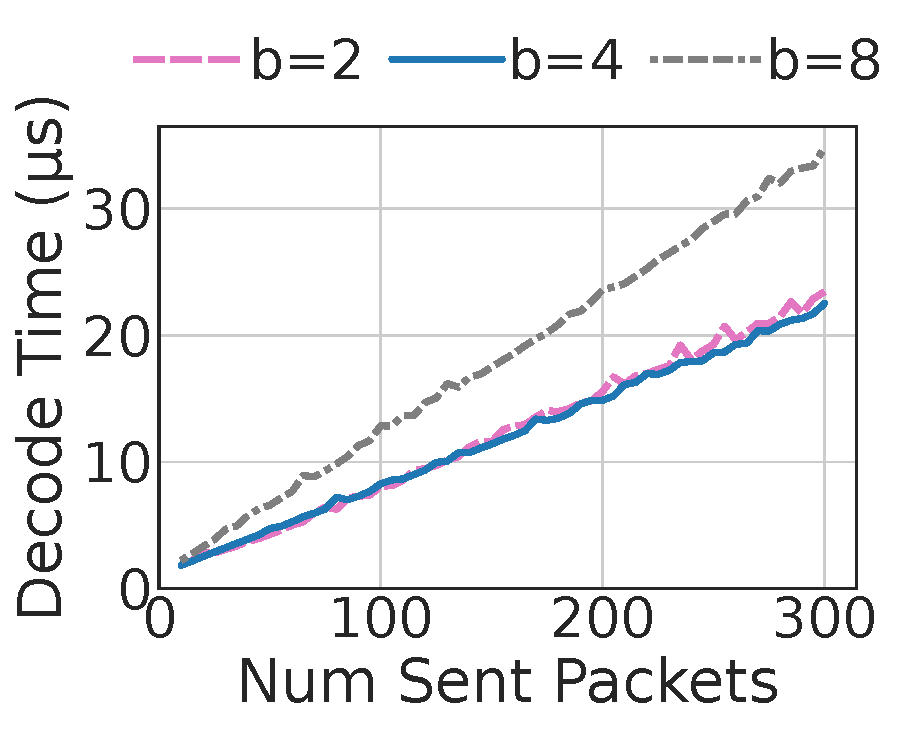
\includegraphics[width=\linewidth,trim={3mm 0 7mm 0},clip]{quack/figures/fig2a_quack_num_candidates_vs_decode_time.pdf}
	\caption{Evaluate a degree-$m=t=10$ polynomial at $n$ candidate roots.}
	\label{fig:quack:psum:n-vs-decoding}
\end{subfigure}
\hspace{-0.1em}
\begin{subfigure}{0.32\columnwidth}
	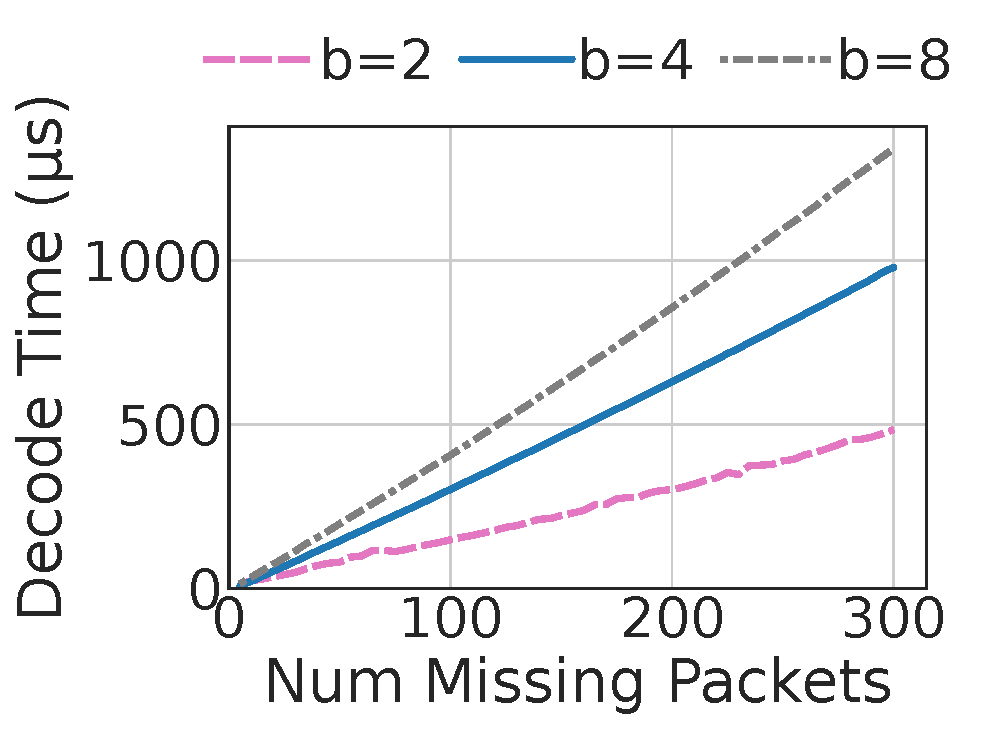
\includegraphics[width=\linewidth,trim={3mm 0 7mm 0},clip]{quack/figures/fig2b_quack_num_missing_vs_decode_time.pdf}
	\caption{Plug $n=300$ candidate roots into a degree-$m$ polynomial.}
	\label{fig:quack:psum:m-vs-decoding}
\end{subfigure}
\hspace{-0.1em}
\begin{subfigure}{0.32\columnwidth}
	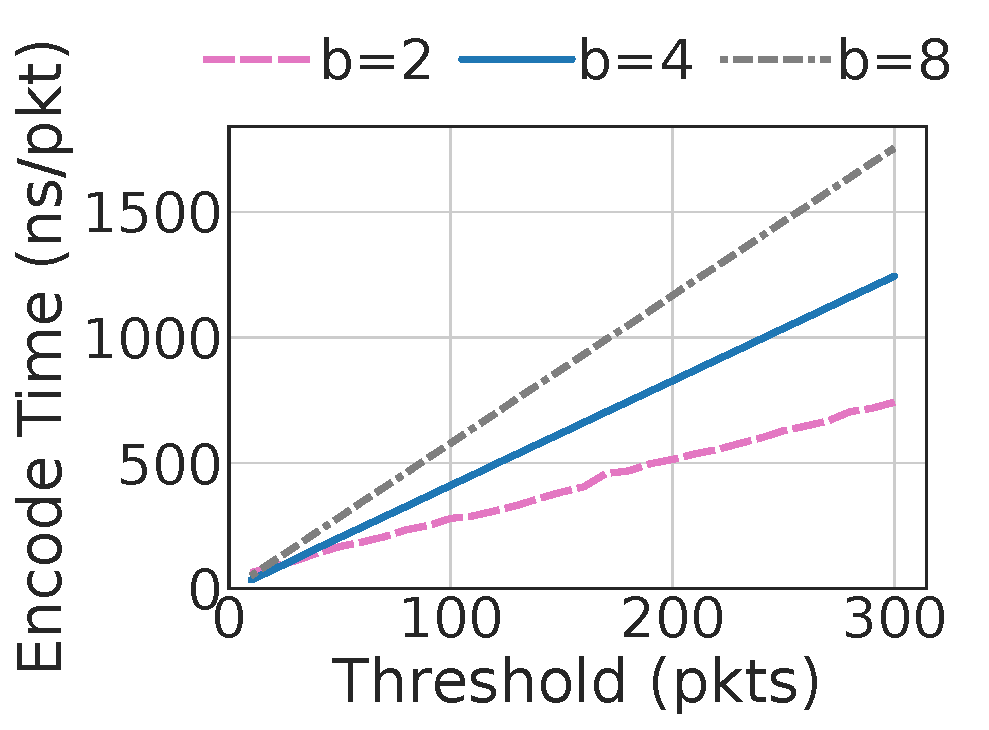
\includegraphics[width=\linewidth,trim={3mm 0 7mm 0},clip]{quack/figures/fig2c_quack_threshold_vs_encode_time.pdf}
	\caption{Update $t$ power sum equations.
	Average of $1000$ packets.}
	\label{fig:quack:psum:construction-time}
\end{subfigure}
\caption{How power sum quACK performance depends on various parameters:
bit width, threshold, number of sent and missing packets.
Average of 100 trials.
}
\label{fig:quack:psum}
\end{figure}


In this section, we benchmark the power sum quACK construction and evaluate the
computation cost for different parameters in packet-scale settings.
We explore different bit widths for the identifier and settle on
using 32-bit packet identifiers.
Our microbenchmarks used an m4.xlarge AWS instance with a 4-CPU Intel Xeon E5
processor @ 2.30 GHz and 16 GB memory.

\subsection{Identifier bit widths}
\label{sec:quack:psum-microbenchmarks:bit-widths}

The more bits we use in an identifier, the less likely that there will be a
collision, but different bit widths have different implications for the
computation cost based on which instructions the CPU can use. Modular
operations are efficient for 16- and 32-bit integers, fitting within the 64-bit
word size (the number of bits that can be processed in one instruction) of most
modern CPUs. For example, to multiply two 32-bit integers, we cast them to
64-bit integers, multiply, then take the modulus.

\Cref{fig:quack:psum} shows the best encoding and decoding times we achieved
at different bit widths, demonstrating that computation cost is generally higher
for higher bit widths, though not significantly. For 16-bit identifiers only, we
precomputed power tables that fit in the L3 cache. For 64-bit identifiers, we
implemented Montgomery modular multiplication~\cite{montgomery1985modular}
to avoid an expensive hardware division for 128-bit integers. In the remainder
of this dissertation, we select $b=4$, or 32-bit identifiers, as the preferred
tradeoff between collision probability, the size of the quACK, and computation
cost.

\subsection{Encoding time}
\label{sec:quack:psum-microbenchmarks:encoding}

Encoding a single packet requires updating the $t$ power sums in the power sum
quACK.
The per-packet encoding time is thus directly proportional to the threshold
number of missing packets $t$ (\Cref{fig:quack:psum:construction-time}) at
$\approx 3$ ns/power sum.
Each power sum can be updated in a constant number of operations based on the
previous power sum, which is a single modular addition and multiplication.

\subsection{Decoding time}
\label{sec:quack:psum-microbenchmarks:decoding}

Decoding the power sum quACK requires finding the solution to a system of power
sum polynomial equations. This boils down to applying Newton's identities (a
linear algorithm) and finding the roots of a polynomial equation in a modular
field~\cite{eppstein2011straggler}.
Factoring a polynomial is asymptotically fast in theory, but the implementation
is branch-heavy and complicated~\cite{parigp2018}.
We find that in practice, it is faster to plug in and determine which of the
$n$ candidate roots evaluate to zero when there are $n < 40,000$ roots.
We use this method to decode the power sum quACK instead of factorization.

The decoding time of this method is directly proportional to the number of
candidate packets $n$ (\Cref{fig:quack:psum:n-vs-decoding})
and the number of missing packets $m$ (\Cref{fig:quack:psum:m-vs-decoding}).
Decoding takes $\approx 11$ ns/candidate/missing, and both $n$ and $m$ are
typically a few hundred at most.
Thus it is typically for encoding to take a few nanoseconds per packet and
decoding to take a few microseconds per quACK.

\section{IBLT microbenchmarks}
\label{sec:quack:iblt-microbenchmarks}

Both constructions of the quACK implement the same interface and can be used
interchangeably, so when should we prefer one to the other? In this section, we
compare the encoding and decoding times of each construction in practice,
including how they scale with the communication cost and the number of missing
packets. We also explore how to configure the IBLT quACK based on its
probabilistic correctness. We run the microbenchmarks on a single core of an
AWS m4.xlarge instance.

\subsection{Encoding and decoding time scalability}
\label{sec:quack:iblt-microbenchmarks:scalability}

\begin{figure}[t]
    \centering
    \begin{subfigure}[b]{0.37\linewidth}
        \centering
        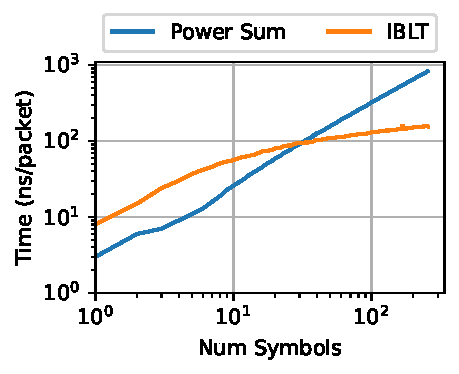
\includegraphics[width=\linewidth]{quack/figures/quack_encode.pdf}
        \caption{Encode time.}
        \label{fig:quack:iblt-computation:encode}
    \end{subfigure}
    \begin{subfigure}[b]{0.37\linewidth}
        \centering
        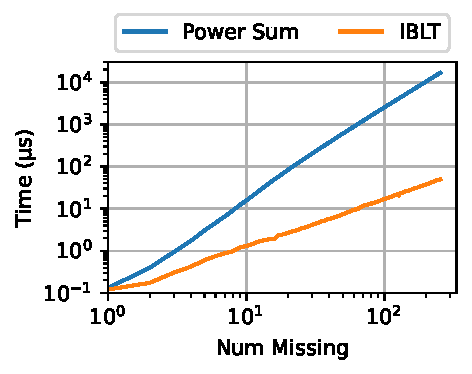
\includegraphics[width=\linewidth]{quack/figures/quack_decode.pdf}
        \caption{Decode time.}
        \label{fig:quack:iblt-computation:decode}
    \end{subfigure}
    \caption{IBLT vs. power sum quACK microbenchmarks. The IBLT quACK is more
     computationally scalable than the power sum quACK, but the encoding time
     suffers from constant factor overheads with a smaller number of symbols.
     The cumulative time of the trials is at least $100$ ms.
     }
    \label{fig:quack:iblt-computation}
\end{figure}

Encoding and decoding operations in the IBLT quACK update a logarithmic number
of symbols per-packet, compared to all of the symbols in the power sum quACK.
This results in better computational complexity in theory, but in practice we
find that the encoding and decoding times also depend on the constant factor
overheads of the pseudorandom mapping algorithm.

The encoding time in the IBLT quACK is faster when there are at least
$\approx\!30$ symbols (\Cref{fig:quack:iblt-computation:encode}).
Each update in the IBLT uses an expensive square root instruction in the
pseudorandom mapping algorithm, adding constant factor overheads that impact
smaller numbers of symbols.

The decoding time is faster for any number of symbols
(\Cref{fig:quack:iblt-computation:decode}).
Note that the power sum quACK actually uses a decoding method that is linear
in \textit{all} packets received, not just the \textit{missing} packets, due to
the complexity of symmetric polynomial factorization.

\subsection{Probabilistic correctness}
\label{sec:quack:iblt-microbenchmarks:correctness}

\begin{figure}[t]
    \centering
    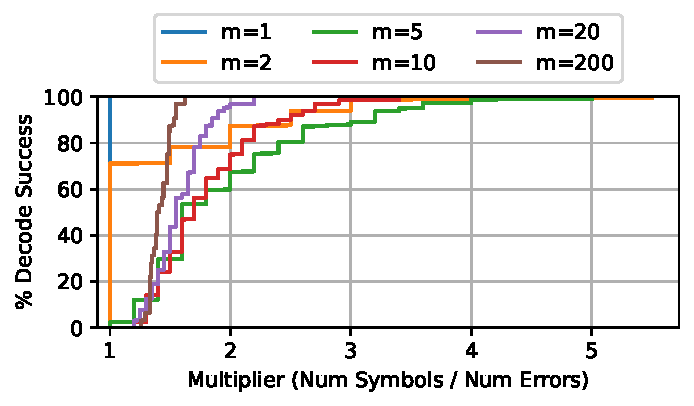
\includegraphics[width=0.9\linewidth]{quack/figures/quack_multiplier.pdf}
    \caption{The CDF of the minimum number of symbols $t$ needed to successfully
    decode an quACK for various numbers of missing packets $m$, 100000 trials.}
    \label{fig:quack:iblt-correctness}
\end{figure}

It is unknown how many symbols are required in the IBLT quACK to decode the same
number of $m$ missing packets using power sums in the previous benchmarks.
There is a constant multiplicative factor on average
($1.23$--$1.35\times$~\cite{yang2024practical,baek2023simple}), but this is
not necessarily representative when $m$ is often small.
\Cref{fig:quack:iblt-correctness} shows the CDF of the minimum number of symbols
to decode various $m$ as this constant multiplier increases. $m=1$ trivially
requires one symbol, while the multiplier decreases for higher $m$ to achieve
the same success rates.

The sender does not know how many symbols it needs to encode to later decode a
certain $m$. Using the power sum quACK, this is exactly $m$ symbols. In the
IBLT quACK, $4 \cdot m$ symbols have at least a $\!98.8\%$ success rate for all
$m$ evaluated in \Cref{fig:quack:iblt-correctness}. When $m$ is large, the IBLT
quACK utilizes more of the link than the power sum quACK, but maintaining more
symbols at the sender and receiver means the sender has a greater worst-case
tolerance for errors with more scalable encoding overheads.

\section{Summary}
\label{sec:quack:summary}

\begin{table*}[ht]
  \centering

  \begin{subtable}[b]{\linewidth}
  \centering
  \begin{tabular}{lccc}
    \toprule
    & \bf Encode Time & \bf Decode Time & \bf QuACK Size \\
    \midrule
    Strawman 1a & $O(1)$ & $O(1)$ & \textcolor{red}{$O(n)$} \\
    Strawman 1b & $O(1)$ & $O(1)$ & \textcolor{red}{$O(n)$} \\
    Strawman 1c & $O(1)$ & $O(1)$ & \textcolor{red}{$O(n)$} \\
    Strawman 2 & $O(1)$ & \textcolor{red}{$O(\binom{n}{t})$} & $O(1)$ \\
    \bf \textcolor{black!50!blue}{Power Sums} & \bf \textcolor{black!50!blue}{$O(t)$} & \bf \textcolor{black!50!blue}{$O(t^2)$} & \bf \textcolor{black!50!blue}{$O(t)$} \\
    \bf \textcolor{black!50!blue}{IBLT} & \bf \textcolor{black!50!blue}{$O(\log t)$} & \bf \textcolor{black!50!blue}{$O(t\log t)$} & \bf \textcolor{black!50!blue}{$O(t)$} \\
    \bottomrule
  \end{tabular}
  \caption{The algorithmic complexity of the costs of each quACK construction.
  $n = |S|$ is the total number of sent elements, $t \geq |S \setminus R|$ is an
  upper bound on the number of missing elements.\\
  }
  \label{tab:quack:overview:theoretical}
  \end{subtable}

  \begin{subtable}[b]{\linewidth}
  \centering
  \begin{tabular}{lcccccc}
    \toprule
    & \bf Encode & \bf Decode & \bf Num & \bf Num & \bf  & \bf Cumu- \\
    & \bf Time & \bf Time & \bf Packets & \bf Bytes & \bf Protocol & \bf lative? \\
    \midrule
    Strawman 1a & N/A & N/A & \textcolor{red}{$500$} & $4$ & UDP & No \\
    Strawman 1b & N/A & N/A & \textcolor{red}{$500$} & $4 \cdot window$ & UDP & No \\
    Strawman 1c & N/A & N/A & \textcolor{red}{$\geq 500$} & $4$ & \textcolor{red}{TCP} & Yes \\
    Strawman 2 & $27$ ns/pkt & \textcolor{red}{$88$ Myears} & $1$ & $36$ & UDP & Yes \\
    \bf \textcolor{black!50!blue}{Power Sums} & \bf \textcolor{black!50!blue}{$26$ ns/pkt} & \bf \textcolor{black!50!blue}{$15.5$ $\mu$s} & \bf \textcolor{black!50!blue}{$1$} & \bf \textcolor{black!50!blue}{$48$} & \bf \textcolor{black!50!blue}{UDP} & \bf \textcolor{black!50!blue}{Yes} \\
    \bf \textcolor{black!50!blue}{IBLT} & \bf \textcolor{black!50!blue}{$42$ ns/pkt} & \bf \textcolor{black!50!blue}{$1.3$ $\mu$s} & \bf \textcolor{black!50!blue}{$1$} & \bf \textcolor{black!50!blue}{$\geq 58$} & \bf \textcolor{black!50!blue}{UDP} & \bf \textcolor{black!50!blue}{Yes} \\
    \bottomrule
  \end{tabular}
  \caption{A concrete realization of the costs of each quACK construction.
  Parameters: $n=500$, $t=10$, and the elements are 32-bit integers.}
  \label{tab:quack:overview:practical}
  \end{subtable}

  \caption{ The computation and communication costs of the power sum and IBLT
  quACK constructions are comparable to or better than those of the strawmen.
  The encoding time includes inserting an element into the data structure that
  represents the quACK(s). The decoding time
   includes finding the elements of either $S \setminus R$ or $R \subseteq S$,
   given the quACK(s) and $S$.}
  \label{tab:quack:overview}
\end{table*}


The power sum and IBLT constructions of the quACK can efficiently refer to and
acknowledge a set of randomly encrypted packets
(\Cref{tab:quack:overview:practical}). These constructions are efficient to
decode, add reasonable link overhead, and are cumulative representations of the
packets seen by the receiver. Compared to Strawman 2, the quACKs can be decoded
with simple computational primitives such as XORs and modular arithmetic. Their
link overheads are proportional only to the number of missing packets between
consecutive quACKs, up to a configurable threshold. In comparison, the link
overhead of Strawman 1 is necessarily proportional to the number of received
packets. Our quACK constructions are also resilient to mis-identifying a
received packet as dropped, in the case a quACK is lost in transmission.

Compared to each other, the IBLT quACK has more scalable computational costs
than the power sum quACK but greater constant factor overheads
(\Cref{tab:quack:overview:theoretical}). We find the IBLT quACK to be more
useful when a large number of symbols is required, such as in settings with
high, bursty loss. However, the power sum quACK is still more efficient when
loss is small or infrequent. In addition, since the power sum quACK is
deterministically correct, it may be simpler to reason about when the threshold
is predictable. Thus both constructions have different tradeoffs to consider.

\section{Appendix: Optimizing the power sum quACK at various bit widths}
\label{sec:quack:appendix}

\begin{table}[ht]
  \centering
  % \renewcommand{\arraystretch}{0.000023}
  \begin{tabular}{lcccrrr}
    \toprule
    \bf     & \bf        & \bf       & \bf        & \bf Per-Packet & \bf Decode & \bf Size\\
    \bf Bits  & \bf NF     & \bf PC    & \bf MM     & \bf Encode Time & \bf Time     & \bf (bytes)\\
    \midrule
    32     &        &       &        & $149$ ns & $3.18$ ms      & 82 \\
    \bf \textcolor{black!50!blue}{32*} & \bf \textcolor{black!50!blue}{x} & & & \bf \textcolor{black!50!blue}{151 ns} & \bf \textcolor{black!50!blue}{102 ${\mu}$s} & \bf \textcolor{black!50!blue}{82} \\
    32     & x      &       & x      & $163$ ns & $130$ ${\mu}$s & 82 \\
    16     & x      &       &        & $137$ ns & $101$ ${\mu}$s & 42 \\
    16*    & x      & x     &        & $57$ ns & $43$ ${\mu}$s & 42 \\
    16     & x      & x     & x      & $84$ ns & $48$ ${\mu}$s & 42 \\
    63     & x      &       &        & $1.14$ ${\mu}$s & $622$ ${\mu}$s & 162 \\
    63*    & x      &       & x      & $159$ ns & $121$ ${\mu}$s & 162 \\
  % 64*    & x      &       & x      & $177$ ns & $132$ ${\mu}$s & 162 \\
    \bottomrule
    % removed factoring except for base 32 case since typically faster
    % removed power table for 64 bit because too large
    % removed both power table + montgomery for 16/32 bit to not combine opts
    % * represents optimal for that bit width
  \end{tabular}
  \caption{Power sum QuACK with different bit widths and optimizations,
  using $n=1000$, $t=20$. The three optimizations are not factoring (NF),
  pre-computation (PC), and Montgomery multiplication (MM).
  *Recommended optimizations for that bit width.}
  \label{tab:optimized-quack}
\end{table}

